\documentclass{beamer}
\usepackage[utf8]{inputenc}

\usetheme{Madrid}
\usecolortheme{default}
\usepackage{amsmath,amssymb,amsfonts,amsthm}
\usepackage{mathtools}
\usepackage{txfonts}
\usepackage{tkz-euclide}
\usepackage{listings}
\usepackage{adjustbox}
\usepackage{tfrupee}
\usepackage{array}
\usepackage{gensymb}
\usepackage{tabularx}
\usepackage{gvv}
\usepackage{lmodern}
\usepackage{circuitikz}
\usepackage{tikz}
\lstset{literate={·}{{$\cdot$}}1 {λ}{{$\lambda$}}1 {→}{{$\to$}}1}
\usepackage{graphicx}

\setbeamertemplate{page number in head/foot}[totalframenumber]

\usepackage{tcolorbox}
\tcbuselibrary{minted,breakable,xparse,skins}

\definecolor{bg}{gray}{0.95}
\DeclareTCBListing{mintedbox}{O{}m!O{}}{%
  breakable=true,
  listing engine=minted,
  listing only,
  minted language=#2,
  minted style=default,
  minted options={%
    linenos,
    gobble=0,
    breaklines=true,
    breakafter=,,
    fontsize=\small,
    numbersep=8pt,
    #1},
  boxsep=0pt,
  left skip=0pt,
  right skip=0pt,
  left=25pt,
  right=0pt,
  top=3pt,
  bottom=3pt,
  arc=5pt,
  leftrule=0pt,
  rightrule=0pt,
  bottomrule=2pt,
  toprule=2pt,
  colback=bg,
  colframe=orange!70,
  enhanced,
  overlay={%
    \begin{tcbclipinterior}
    \fill[orange!20!white] (frame.south west) rectangle ([xshift=20pt]frame.north west);
    \end{tcbclipinterior}},
  #3,
}
\lstset{
    language=C,
    basicstyle=\ttfamily\small,
    keywordstyle=\color{blue},
    stringstyle=\color{orange},
    commentstyle=\color{green!60!black},
    numbers=left,
    numberstyle=\tiny\color{gray},
    breaklines=true,
    showstringspaces=false,
}

\title{12.27}
\date{October 6, 2025}
\author{Bhargav - EE25BTECH11013}

\begin{document}

\frame{\titlepage}

\begin{frame}{Question}
\textbf{Question}: \\
1200 men and 500 women can build a bridge in 2 weeks. 900 men and 250 women will take 3 weeks to build the same bridge. How many men will be needed to build the bridge in one week? \\
\end{frame}
\begin{frame}{Solution}
Let one man complete work in X weeks and one woman complete work in Y weeks\\
In one week a man can complete $\frac{1}{X}$ work and woman can complete $\frac{1}{Y}$
\begin{align}
\frac{1200}{X} + \frac{500}{Y} = \frac{1}{2} \implies XY - 1000X - 2400Y = 0 \label{eq:1}
\end{align}
\begin{align}
\frac{900}{X} + \frac{250}{Y} = \frac{1}{3} \implies XY - 750X - 2700Y = 0 \label{eq:2}
\end{align}

\end{frame}

\begin{frame}{Solution}
Rotate the axis by $45\degree$ to remove the $XY$ term in the equations
\begin{align}
\vec{X} = \vec{Q}\vec{x} 
\end{align}
(where $\vec{Q}$ is the rotation matrix)
\begin{align}
\myvec{X \\ Y} = \myvec{\frac{1}{\sqrt{2}} & \frac{1}{\sqrt{2}} \\ \frac{1}{\sqrt{2}} & -\frac{1}{\sqrt{2}}}\myvec{x \\ y} \label{eq:3}
\end{align}
\begin{align}
\implies XY = \frac{x^2 - y^2}{2}
\end{align}
The conic equations become:
\begin{align}
x^2 - y^2 -3400\sqrt{2}x + 1400\sqrt{2}y = 0
\end{align}
\begin{align}
x^2 - y^2 - 3450\sqrt{2}x + 1950\sqrt{2}y = 0
\end{align}

\end{frame}

\begin{frame}{Solution}
These can be represented as general conic equations:
\begin{align}
\vec{x}^\top\vec{V}\vec{x} + 2\vec{u}^\top\vec{x} + f = 0
\end{align}\\ \\ \\ 
For the conics: $\vec{V} = \myvec{1 & 0 \\ 0 & -1}$, $\vec{u_1} = \myvec{-1700\sqrt{2} \\ 700\sqrt{2}}$, $\vec{u_2} = \myvec{-1725\sqrt{2} \\ 975\sqrt{2}}$, $f=0$

In homogeneous coordinates, using the form $\vec{x}^\top C \vec{x} = 0$, where $\vec{x} = \myvec{x & y & 1}^T$, the matrices for the conics are:\\
\begin{align}
\vec{C} = \myvec{\vec{V} & \vec{u^T} \\ \vec{u} & f}
\end{align}
  
\end{frame}

\begin{frame}{Solution}
\begin{align}
\implies \vec{C_1} = \myvec{1 & 0 & -1700\sqrt{2} \\ 0 & -1 & 700\sqrt{2} \\ -1700\sqrt{2} & 700\sqrt{2} & 0}
\end{align}
\begin{align}
\implies \vec{C_2} = \myvec{1 & 0 & -1725\sqrt{2} \\ 0 & -1 & 975\sqrt{2} \\ -1725\sqrt{2} & 975\sqrt{2} & 0}
\end{align}\\    
The intersection point of both the conics lies on the conic formed by their individual linear combination $\vec{C(\mu)} = \vec{C_1} + \mu\vec{C_2}$. We must find the value of $\mu$ that makes the determinant of the conic's matrix as 0.

\end{frame}

\begin{frame}{Solution}
\begin{align}
\vec{C(\mu)} = \myvec{1+\mu & 0 & -1700\sqrt{2} -1725\sqrt{2}\mu \\ 0 & -\mu - 1 & 700\sqrt{2}+  975\sqrt{2}\mu \\ -1700\sqrt{2} -1725\sqrt{2}\mu & 700\sqrt{2}+ 975\sqrt{2}\mu & 0}
\end{align}
On solving $\det{\brak{\vec{C(\mu)}}}$ = 0, the simplest value of $\mu = -1$
\begin{align}
\brak{\vec{x}^\top\vec{V}\vec{x} + 2\vec{u_1}^\top\vec{x} + f} + \brak{-1}\brak{\vec{x}^\top\vec{V}\vec{x} + 2\vec{u_2}^\top\vec{x} + f} = 0
\end{align}
The chord of intersection of the 2 hyperbolas is:
\begin{align}
\vec{\brak{u_1^T - u_2^T}}\vec{x} = 0 \implies \myvec{1 & -11}\myvec{x \\ y} = 0
\end{align}

\end{frame}

\begin{frame}{Solution}
The point of intersection of the common chord and the first hyperbola can be found out by solving them
\begin{align}
\vec{x} = \vec{h} + k_i\vec{m}, \vec{h} = \myvec{0 \\ 0}, \vec{m} = \myvec{11 \\ 1}
\end{align}

\begin{align}
(\vec{h} + k_i \vec{m})^{\top} \vec{V} (\vec{h} + k_i \vec{m}) + 2\vec{u}^{\top} (\vec{h} + k_i \vec{m}) + f &= 0 \\
\implies k_i^{2} \vec{m}^{\top}\vec{V}\vec{m} + 2k_i \vec{m}^{\top} (\vec{V}\vec{h} + \vec{u}) + \vec{h}^{\top}\vec{V}\vec{h} + 2\vec{u}^{\top}\vec{h} + f &= 0 \\
\text{or, } k_i^{2} \vec{m}^{\top}\vec{V}\vec{m} + 2k_i \vec{m}^{\top} (\vec{V}\vec{h} + \vec{u}) + g(\vec{h}) &= 0
\end{align}

\end{frame}

\begin{frame}{Solution}
Solving the above quadratic gives the equation
\begin{align}
k_i = \frac{1}{\vec{m}^{\top}\vec{V}\vec{m}}
\brak{
    -\vec{m}^{\top} (\vec{V}\vec{h} + \vec{u})
    \;\pm\;
    \sqrt{ \sbrak{\vec{m}^{\top}(\vec{V}\vec{h} + \vec{u})}^2
    - g(\vec{h}) \, (\vec{m}^{\top}\vec{V}\vec{m}) }
    }
\end{align}
Solving we get:
\begin{align}
k_1 = 0, k_2 = 300\sqrt{2}
\end{align}

The point of intersection:
\begin{align}
\vec{x_1} = \myvec{0 \\ 0}, \vec{x_2} = \myvec{3300\sqrt{2} \\ 300\sqrt{2}}
\end{align}
The point $\vec{x_1} = \myvec{0 \\ 0}$ is not possible because it causes division by 0.\\
\end{frame}
\begin{frame}{Solution}
Substituting $\vec{x_2}$ in the rotation matrix equation:
\begin{align}
\vec{X} = \myvec{3600 \\ 3000}
\end{align}
A man can complete the work in 3600 weeks, a woman can complete the work in 3000 weeks
\end{frame}
\begin{frame}{Plot}

\begin{figure}[h!]
    \centering
    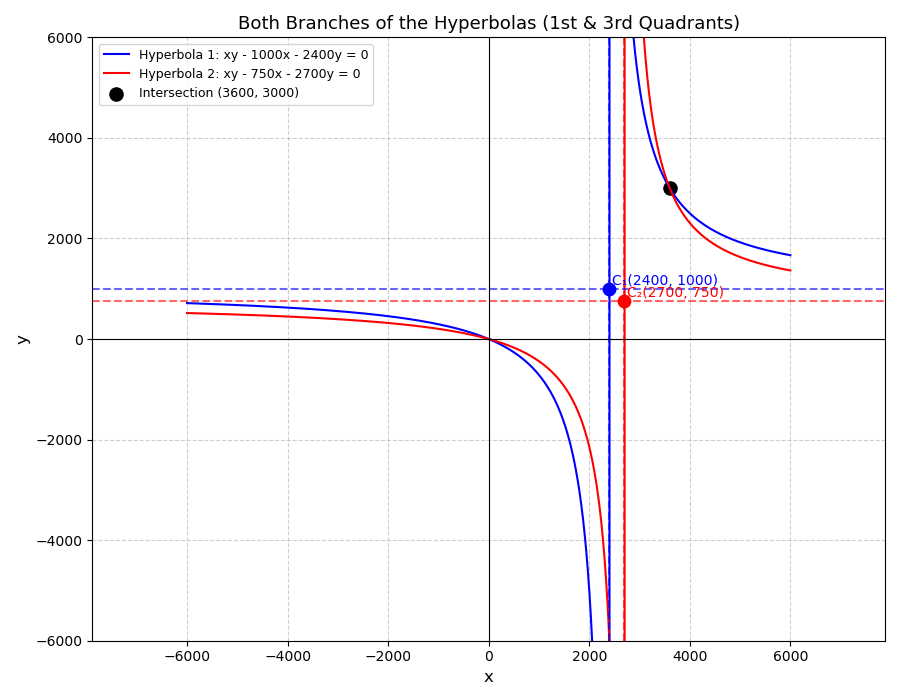
\includegraphics[height=0.5\textheight, keepaspectratio]{figs/Figure_1.png}
    \label{figure_1}
\end{figure}
\end{frame} 



\begin{frame}[fragile]
    \frametitle{C Code}
    \begin{lstlisting}

#include <stdio.h>

double determinant3(double A[3][3]) {
    double det =
        A[0][0]*(A[1][1]*A[2][2] - A[1][2]*A[2][1]) -
        A[0][1]*(A[1][0]*A[2][2] - A[1][2]*A[2][0]) +
        A[0][2]*(A[1][0]*A[2][1] - A[1][1]*A[2][0]);
    return det;
}


    \end{lstlisting}
\end{frame}
\begin{frame}[fragile]
    \frametitle{Python + C Code}
    \begin{lstlisting}
import numpy as np
import matplotlib.pyplot as plt
import ctypes

lib = ctypes.CDLL("./libcode.so")
lib.determinant3.restype = ctypes.c_double

# Example use of determinant from C
A = ((ctypes.c_double * 3) * 3)()
data = [
    [1, 2, 3],
    [0, 1, 4],
    [5, 6, 0]
]
for i in range(3):
    for j in range(3):
        A[i][j] = data[i][j]

det_val = lib.determinant3(A)
    \end{lstlisting}
\end{frame}
\begin{frame}[fragile]
    \frametitle{Python + C Code}
    \begin{lstlisting}
print("Determinant (computed in C):", det_val)
def hyperbola1(x):
    return (1000 * x) / (x - 2400)

def hyperbola2(x):
    return (750 * x) / (x - 2700)

center1 = (2400, 1000)
center2 = (2700, 750)
intersection = (3600, 3000)

# Plot both branches
x_vals = np.linspace(-6000, 6000, 2000)
x_vals1 = x_vals[x_vals != 2400]
x_vals2 = x_vals[x_vals != 2700]

y1 = hyperbola1(x_vals1)
y2 = hyperbola2(x_vals2)


    \end{lstlisting}
\end{frame}
\begin{frame}[fragile]
    \frametitle{Python + C Code}
    \begin{lstlisting}
plt.figure(figsize=(9, 7))

plt.plot(x_vals1, y1, 'b', label='Hyperbola 1: xy - 1000x - 2400y = 0')
plt.plot(x_vals2, y2, 'r', label='Hyperbola 2: xy - 750x - 2700y = 0')

# Centers and asymptotes
plt.scatter(*center1, color='blue', s=70)
plt.scatter(*center2, color='red', s=70)
plt.axvline(x=2400, color='b', linestyle='--', alpha=0.6)
plt.axhline(y=1000, color='b', linestyle='--', alpha=0.6)
plt.axvline(x=2700, color='r', linestyle='--', alpha=0.6)
plt.axhline(y=750, color='r', linestyle='--', alpha=0.6)

# Intersection
plt.scatter(*intersection, color='black', s=90, label='Intersection (3600,3000)')
plt.text(intersection[0]+80, intersection[1]+80, f"({intersection[0]}, {intersection[1]})", fontsize=10)




    \end{lstlisting}
\end{frame}
\begin{frame}[fragile]
    \frametitle{Python + C Code}
    \begin{lstlisting}
# Formatting
plt.title("Hyperbolas in Original Coordinates (1st & 3rd Quadrants)", fontsize=13)
plt.xlabel("x")
plt.ylabel("y")
plt.grid(True, linestyle='--', alpha=0.6)
plt.axhline(0, color='k', linewidth=0.8)
plt.axvline(0, color='k', linewidth=0.8)
plt.axis('equal')
plt.xlim(-6000, 6000)
plt.ylim(-6000, 6000)
plt.legend(fontsize=9, loc='upper left')
plt.tight_layout()
plt.savefig("/mnt/c/Users/bharg/Documents/backupmatrix/ee25btech11013/matgeo/12.27/figs/Figure_1.png")

plt.show()




    \end{lstlisting}
\end{frame}
\begin{frame}[fragile]
    \frametitle{Python Code}
    \begin{lstlisting}
import numpy as np
import matplotlib.pyplot as plt

def hyperbola1(x):
    # From: xy - 1000x - 2400y = 0  =>  y = 1000x / (x - 2400)
    return (1000 * x) / (x - 2400)

def hyperbola2(x):
    # From: xy - 750x - 2700y = 0  =>  y = 750x / (x - 2700)
    return (750 * x) / (x - 2700)

# Centers (from completing the product form)
center1 = (2400, 1000)
center2 = (2700, 750)

x1 = np.linspace(-6000, 6000, 2000)

# Avoid division by zero at vertical asymptotes
x1 = x1[x1 != 2400]
x2 = x1[x1 != 2700]



    \end{lstlisting}
\end{frame}
\begin{frame}[fragile]
    \frametitle{Python Code}
    \begin{lstlisting}
y1 = hyperbola1(x1)
y2 = hyperbola2(x1)

plt.figure(figsize=(9, 7))

# Plot both hyperbolas
plt.plot(x1, y1, 'b', label='Hyperbola 1: xy - 1000x - 2400y = 0')
plt.plot(x1, y2, 'r', label='Hyperbola 2: xy - 750x - 2700y = 0')

# Plot asymptotes for each hyperbola
plt.axvline(x=2400, color='b', linestyle='--', alpha=0.6)
plt.axhline(y=1000, color='b', linestyle='--', alpha=0.6)
plt.axvline(x=2700, color='r', linestyle='--', alpha=0.6)
plt.axhline(y=750, color='r', linestyle='--', alpha=0.6)

# Plot centers
plt.scatter(*center1, color='blue', s=80, zorder=10)
plt.text(center1[0]+50, center1[1]+80, f"C₁({center1[0]}, {center1[1]})", fontsize=10, color='blue')

    \end{lstlisting}
\end{frame}
\begin{frame}[fragile]
    \frametitle{Python Code}
    \begin{lstlisting}
plt.scatter(*center2, color='red', s=80, zorder=10)
plt.text(center2[0]+50, center2[1]+80, f"C₂({center2[0]}, {center2[1]})", fontsize=10, color='red')
intersection = (3600, 3000)
plt.scatter(*intersection, color='black', s=90, label=f'Intersection {intersection}')
plt.title("Both Branches of the Hyperbolas (1st & 3rd Quadrants)", fontsize=13)
plt.xlabel("x", fontsize=12)
plt.ylabel("y", fontsize=12)
plt.grid(True, linestyle='--', alpha=0.6)
plt.axhline(0, color='k', linewidth=0.8)
plt.axvline(0, color='k', linewidth=0.8)
plt.legend(fontsize=9, loc='upper left')
plt.axis('equal')
plt.xlim(-6000, 6000)
plt.ylim(-6000, 6000)
plt.tight_layout()
plt.savefig("/mnt/c/Users/bharg/Documents/backupmatrix/ee25btech11013/matgeo/12.27/figs/Figure_1.png")
plt.show()




    \end{lstlisting}
\end{frame}


\end{document}

